%%%%%%%%%%%%%%%%%%% 
% RELATION EXTRACTION
%%%%%%%%%%%%%%%%%%%
\begin{frame}{What's Missing?}
\hh{There's more to life than extracting 41 relations}
\begin{center}
  
\includegraphics[height=4cm]{../img/bartwindow.png} \\

  \pause
  \w{Rainbows are caused by the sun} \\
  \w{Cars drive on roads} \\
  \pause
  \w{Obama gave a speech on healthcare} \\
  \w{$\dots$}

\end{center}
\end{frame}

\begin{frame}{What's Missing?}
\hh{There's more to life than extracting 41 relations} \\
\hh{``High'' recall (0.29), but low precision (0.36)} \\
\begin{center}
  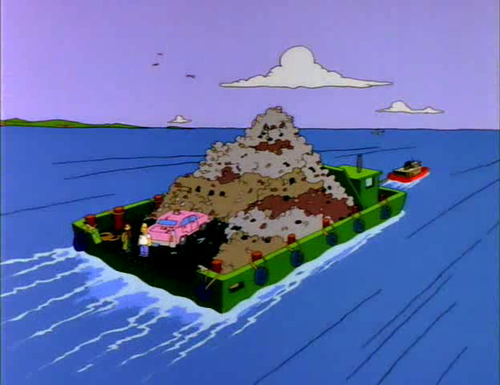
\includegraphics[height=4cm]{../img/simpsons-garbage.png} \\
  \textcolor{white}{Simpsons} \\
  \textcolor{white}{Simpsons} \\
\end{center}
\end{frame}

\begin{frame}{What's Missing?}
\hh{There's more to life than extracting 41 relations} \\
\hh{``High'' recall (0.29), but low precision (0.36)} \\
\hh{Easy to throw off with logical subtleties}
\begin{center}
  
\includegraphics[height=4cm]{../img/bart-chalkboard.png} \\
  \textcolor{white}{Simpsons} \\
\end{center}
\end{frame}

\begin{frame}{What's Missing?}
\hh{There's more to life than extracting 41 relations} \\
\hh{``High'' recall (0.29), but low precision (0.36)} \\
\hh{Easy to throw off with logical subtleties}
\begin{center}
  
\includegraphics[height=4cm]{../img/bart-chalkboard.png}
  \textcolor{white}{123}
  
\includegraphics[height=4cm]{../img/bart-dentist.jpg} \\
  \textcolor{white}{Simpsons} \\
\end{center}
\end{frame}


%%%%%%%%%%%%%%%%%%% 
% ENTAILMENT
%%%%%%%%%%%%%%%%%%%
\begin{frame}{ACL 2015: Treat As Entailment}
\begin{center}
  \w{Born in a small town, she took the midnight train going anywhere.} \\ 
  $\implies$ \w{She was born in small town.} \\
  $\implies$ (\w{She}; \w{was born in}; \w{small town.}) \\
\end{center}
\pause

\hh{Problem 1:} Long sentences are hard to handle:
\begin{center}
  \begin{dependency}[text only label, label style={above}]
    \begin{deptext}[column sep=-0.00cm]
      Born \& in \& a \& small \& town \&[-1ex] , \& she \& took \& the \&
        midnight \& train \& going \& anywhere \&[-1ex] . \\
    \end{deptext}
    \depedge[edge unit distance=1.75ex]{1}{5}{prep\_in}
    \depedge[edge unit distance=1.5ex]{5}{4}{amod}
    \depedge[edge unit distance=2.25ex]{5}{3}{det}
    \depedge[edge unit distance=1.5ex, edge style={darkred!60!black,thick,densely dotted}]{8}{1}{\textbf{\darkred{vmod}}}
    \depedge[edge unit distance=2.5ex, edge style={blue!60!black,thick}]{8}{7}{\darkblue{nsubj}}
    \depedge[edge unit distance=2.25ex]{8}{11}{dobj}
    \depedge[edge unit distance=1.5ex]{11}{10}{nn}
    \depedge[edge unit distance=1.9ex]{11}{9}{det}
    \depedge[edge unit distance=1.5ex]{11}{12}{vmod}
    \depedge[edge unit distance=1.5ex]{12}{13}{dobj}
  \end{dependency}
\end{center}
\pause

\hh{Problem 2:} We'd like to be aware of logical subtleties:
\begin{center}
  \w{All young rabbits drink milk} \\ 
  $\centernot \implies$ \w{All rabbits drink milk}
\end{center}
\end{frame}


%%%%%%%%%%%%%%%%%%% 
% CLAUSE SPLITTING
%%%%%%%%%%%%%%%%%%%
\begin{frame}{Solving Problem 1: Clause Splitting}
\hh{Step 1:} Split sentence into clauses
\begin{itemize}
  \item[]
    \begin{dependency}[text only label, label style={above}]
      \begin{deptext}[column sep=-0.00cm]
        Born \& in \& a \& small \& town \&[-1ex] , \& she \& took \& the \&
          midnight \& train \& going \& anywhere \&[-1ex] . \\
      \end{deptext}
      \depedge[edge unit distance=1.25ex]{1}{5}{prep\_in}
      \depedge[edge unit distance=1.0ex]{5}{4}{amod}
      \depedge[edge unit distance=1.4ex]{5}{3}{det}
      \depedge[edge unit distance=1.0ex, edge style={darkred!60!black,thick,densely dotted}]{8}{1}{\textbf{\darkred{vmod}}}
      \depedge[edge unit distance=2.0ex, edge style={blue!60!black,thick}]{8}{7}{\darkblue{nsubj}}
      \depedge[edge unit distance=1.75ex]{8}{11}{dobj}
      \depedge[edge unit distance=1.0ex]{11}{10}{nn}
      \depedge[edge unit distance=1.4ex]{11}{9}{det}
      \depedge[edge unit distance=1.0ex]{11}{12}{vmod}
      \depedge[edge unit distance=1.0ex]{12}{13}{dobj}
    \end{dependency}

  \item[]
      \begin{dependency}[text only label, label style={above}]
        \begin{deptext}[column sep=-0.05cm]
          she \& Born \& in \& a \& small \& town \\
        \end{deptext}
        \depedge[edge unit distance=1.25ex]{2}{6}{prep\_in}
        \depedge[edge unit distance=1.0ex]{6}{5}{amod}
        \depedge[edge unit distance=1.4ex]{6}{4}{det}
        \depedge[edge unit distance=2.0ex, edge style={blue!60!black,thick}]{2}{1}{\darkblue{nsubj}}
      \end{dependency}
\end{itemize}
\pause

\hh{Approach:} Train classifier for whether a dependency arc is a clause.
\end{frame}


%%%%%%%%%%%%%%%%%%% 
% SENTENCE SHORTENING
%%%%%%%%%%%%%%%%%%%
\begin{frame}{Solving Problem 1: Clause Splitting}
\hh{Step 1:} Split sentence into clauses \\
\hh{Step 2:} Shorten each clause:
\vspace{2em}
\begin{itemize}
  \item[]
      \begin{dependency}[text only label, label style={above}]
        \begin{deptext}[column sep=-0.05cm]
          she \& Born \& in \& a \& small \& town \\
        \end{deptext}
        \depedge[edge unit distance=1.25ex]{2}{6}{prep\_in}
        \depedge[edge unit distance=1.0ex]{6}{5}{amod}
        \depedge[edge unit distance=1.4ex]{6}{4}{det}
        \depedge[edge unit distance=2.0ex, edge style={blue!60!black,thick}]{2}{1}{\darkblue{nsubj}}
      \end{dependency}
  \pause
  \item[] $\implies$ \w{She born in a small town}
  \item[] $\implies$ \w{She born in small town}
  \item[] $\implies$ \w{She born in town}
\end{itemize}
\pause

\hh{Approach:} Natural logic inference (more on this later!)
\end{frame}


%%%%%%%%%%%%%%%%%%% 
% RELATION EXTRACTION
%%%%%%%%%%%%%%%%%%%
\begin{frame}{Solving Problem 1: Clause Splitting}
\hh{Step 1:} Split sentence into clauses \\
\hh{Step 2:} Shorten each clause \\
\hh{Step 3:} Extract relation triples: \\
\pause

\vspace{1em}
\hh{Approach:} 6 easy patterns (and 8 nominal patterns) cover most cases:

\begin{center}
  \begin{tabular}{l|l}
  \textbf{Input} & \textbf{Extraction} \\
  \hline
  \ww{\small{cats play with yarn}}        & \small{(cats; play with; yarn)} \\
  \ww{\small{fish like to swim}}          & \small{(fish; like to; swim)} \\
  \ww{\small{cats have tails}}            & \small{(cats; have; tails)} \\
  \ww{\small{cats are cute}}              & \small{(cats; are; cute)} \\
  \ww{\small{Tom and Jerry are fighting}} & \small{(Tom; fighting; Jerry)} \\
  \ww{\small{There are cats with tails}}  & \small{(cats; have; tails)}
  \end{tabular}
\end{center}
\end{frame}


%%%%%%%%%%%%%%%%%%% 
% RELATION EXTRACTION
%%%%%%%%%%%%%%%%%%%
\begin{frame}{Evaluation on KBP}
\hh{Recall our goals:}
\begin{enumerate}
  \item Open domain relations.
\end{enumerate}
\vspace{1em}
\pause


%%%%%%%%%%%%%%%%%%% 
% MAPPING
%%%%%%%%%%%%%%%%%%%
\hh{Learn a mapping to KBP relations}
\begin{itemize}
  \item Thresholded PMI$^2$ between open domain and KBP relation.
\end{itemize}


\begin{center}
\begin{tabular}{llc}
  \textbf{KBP Relation} & \textbf{Open IE Relation} & \textbf{PMI$^2$} \\
  \hline
  \small{\rel{Org:Founded}}     & \ww{found in} & 1.17             \\
  \small{\rel{Org:Dissolved}}   & \ww{*buy Chrysler in} & 0.95     \\
  \small{\rel{Org:LOC\_Of\_HQ}} & \ww{in} & 2.12                   \\
  \small{\rel{Per:Date\_Of\_Birth}} & \ww{be bear on} & 1.83       \\
  \small{\rel{Per:Loc\_Of\_Death}} & \ww{*elect president of} & 2.89 \\
\end{tabular}
\end{center}

\end{frame}


%%%%%%%%%%%%%%%%%%% 
% RESULTS
%%%%%%%%%%%%%%%%%%%
\begin{frame}{Evaluation on KBP}
\hh{Recall our goals:}
\begin{enumerate}
  \item Open domain relations.
  \item High precision.
  \pause
  \item Respect logical subtleties.
  \begin{itemize}
    \item[] (KBP is the wrong evaluation for this -- stay tuned!)
  \end{itemize}
\end{enumerate}
\vspace{1em}
\pause

\def\bell{\raisebox{-2.5mm}{
\includegraphics[height=5mm]{../img/bell.png}}}
\def\whistle{\raisebox{-2.5mm}{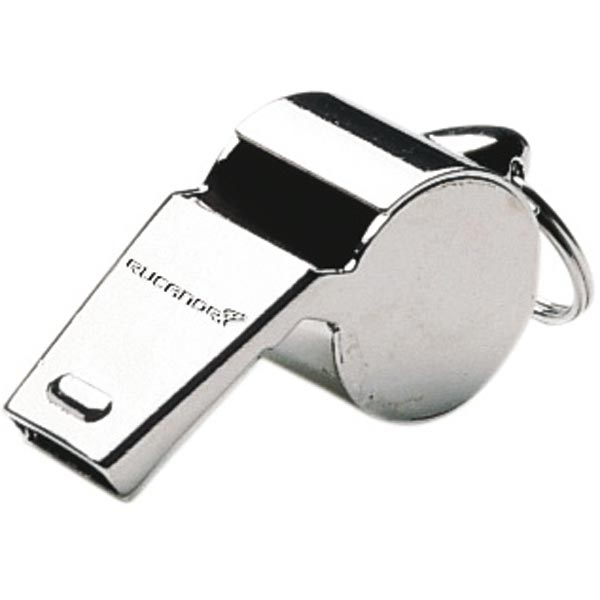
\includegraphics[height=5mm]{../img/whistle.jpg}}}
\begin{center}
\begin{tabular}{lrrr}
\hline
\textbf{System}                & \multicolumn{1}{c}{\textbf{P}}    
                               & \multicolumn{1}{c}{\textbf{R}}    
                               & \multicolumn{1}{c}{\textbf{F$_1$}} \\
\hline
Our System        & 61.9          & 13.9          & 22.7 \\
\hline
\pause
Ollie             & 57.7          & 11.8          & 19.6 \\
UW Submission     & 69.8          & 11.4          & 19.6 \\
\hline
\pause
Our System + \bell\ + \whistle  & 58.6          & 18.6          & 28.3 \\
MIML-RE                        & 39.4          & 36.2          & 37.7 \\
\hline
\end{tabular}
\end{center}

\end{frame}
